% Created 2015-01-09 Fri 13:53
\documentclass[11pt]{article}
\usepackage[utf8]{inputenc}
\usepackage[T1]{fontenc}
\usepackage{fixltx2e}
\usepackage{graphicx}
\usepackage{longtable}
\usepackage{float}
\usepackage{wrapfig}
\usepackage{soul}
\usepackage{textcomp}
\usepackage{marvosym}
\usepackage{wasysym}
\usepackage{latexsym}
\usepackage{amssymb}
\usepackage{hyperref}
\tolerance=1000
\providecommand{\alert}[1]{\textbf{#1}}

\title{Homework 8 Redo}
\author{Nooreen Dabbish}
\date{\today}
\hypersetup{
  pdfkeywords={},
  pdfsubject={},
  pdfcreator={Emacs Org-mode version 7.9.3f}}

\begin{document}

\maketitle

\section{Example of Org-Babel for R Literate Programming}
\label{sec-1}
\subsection{R text output}
\label{sec-1-1}

A simple summary. 




\begin{verbatim}
plot(matrix(rnorm(100), ncol=2), type="l")
\end{verbatim}




\begin{verbatim}
x <- 1:10
library(ascii)
options(asciiType="org")
ascii(summary(table(1:4, 1:4)))
\end{verbatim}

\begin{verbatim}
 - Number of cases in table: 4 
 - Number of factors: 2 
 - Test for independence of all factors:
   - Chisq = 12, df = 9, p-value = 0.2133
   - Chi-squared approximation may be incorrect
\end{verbatim}
\subsection{R graphics output}
\label{sec-1-2}

Note we use the object \texttt{x} generated in previous code block, thanks to
the header option \texttt{:session *R*}.  The output graphics file is
\texttt{a.png}. 





\begin{figure}[p]
\centering
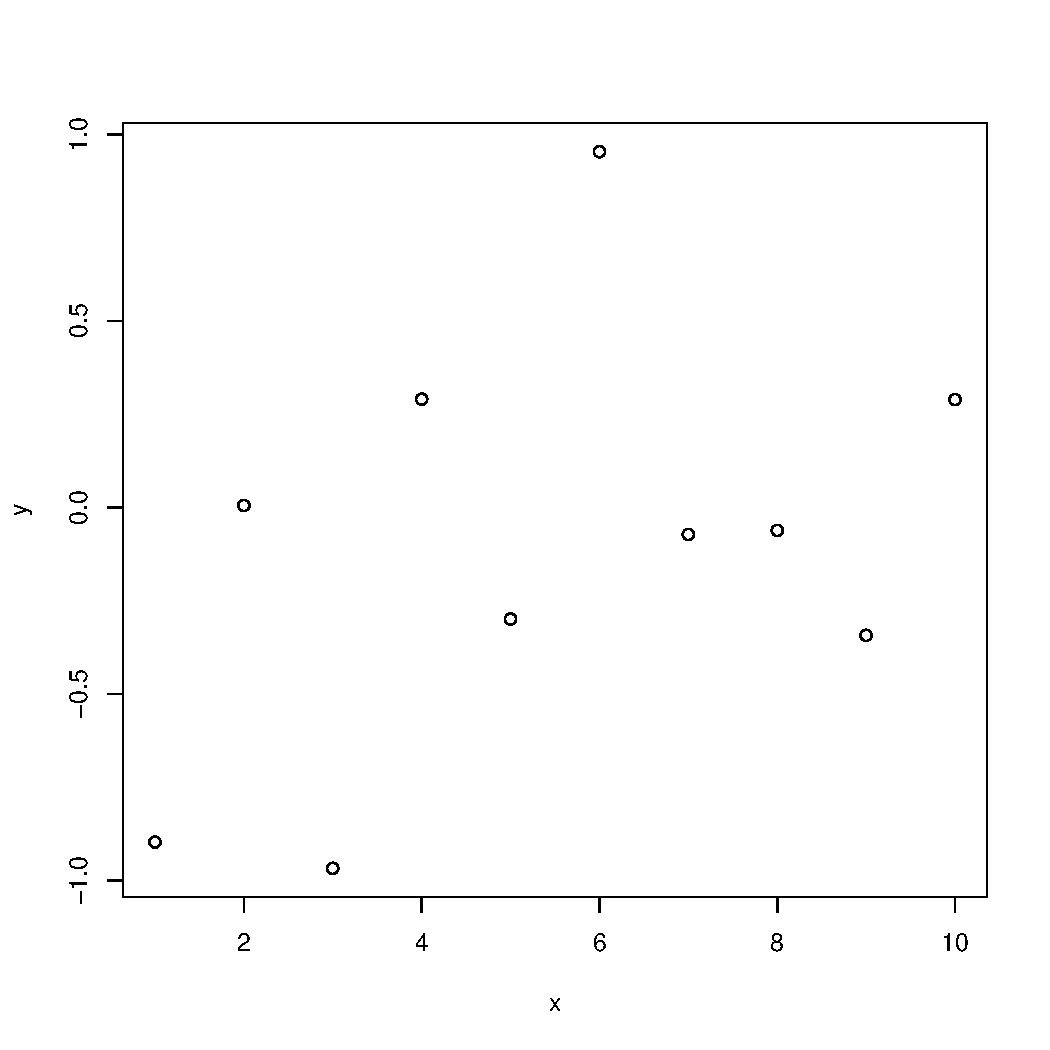
\includegraphics[width=0.8\textwidth,]{a.pdf}
\caption{\label{fig:one}Scatter Plot with Regression Line}
\end{figure}

Same plot with larger dimension:



\begin{figure}[p]
\centering
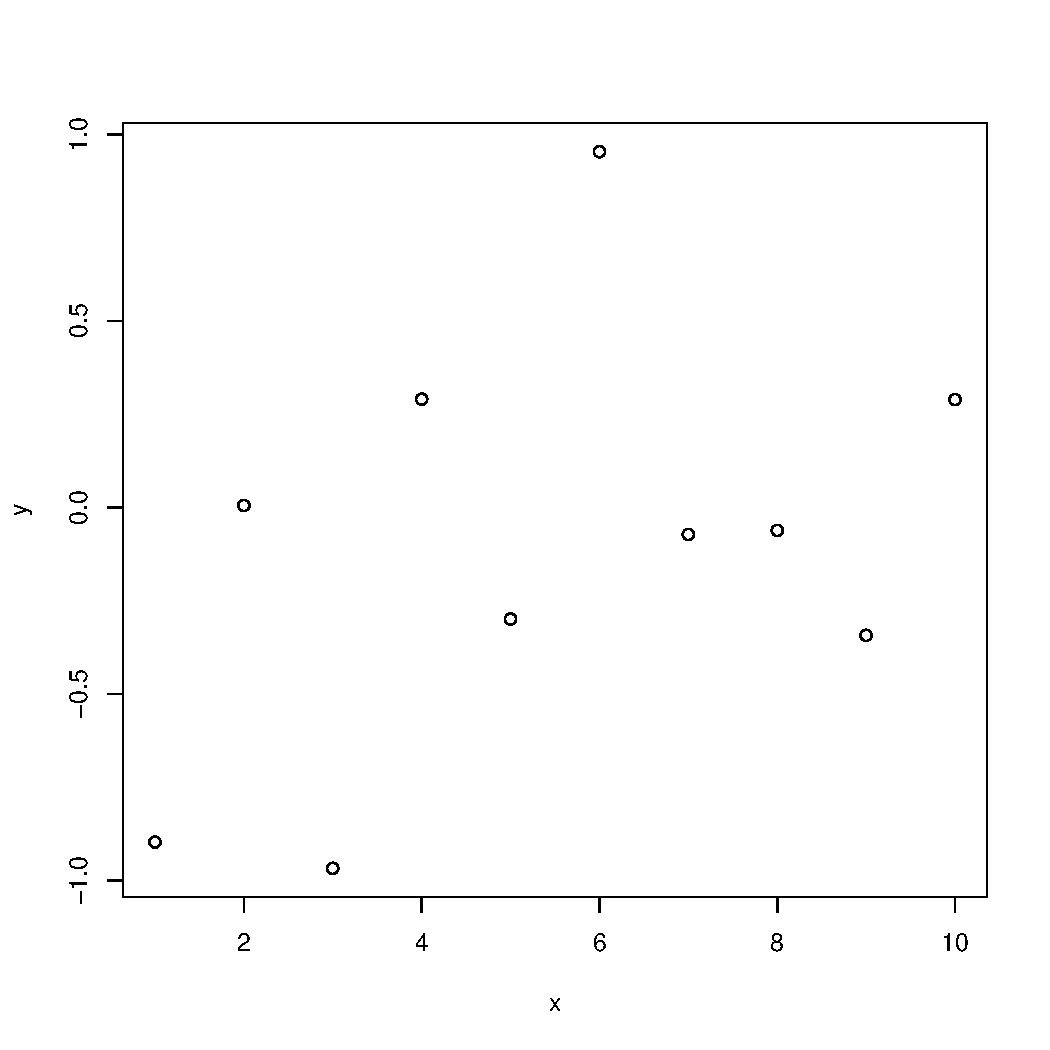
\includegraphics[width=0.8\textwidth,]{b.pdf}
\caption{\label{fig:one}Scatter Plot with Regression Line}
\end{figure}
\section{Problem 1}
\label{sec-2}

$\mu_{0} = 3.35$ percent butterfat\\
$\sigma = 0.15$
\subsection{Find the rejection region at the significance level $\alpha$ = 0.05}
\label{sec-2-1}

\begin{align*}
H_{0}&:\, \mu = \mu_{0} = 3.35\\
H_{A}&:\, \mu \neq \mu_{0}\\
\alpha &= \mathrm{P}(\mathrm{Accept } H_{0} \mid H_{0} \mathrm{ true})\\
       &= \mathrm{P}(z_{\frac{\alpha}{2}} < Z < z_{1 - \frac{\alpha}{2}} \mid \mu=\mu_{0}})\\
       &(=SRC_R[:exports results raw]{round(qnorm(.025),2)}=< Z < =1.96=)
\end{align*}  
y
(-1.96< Z < 1.96)
\section{Problem 2}
\label{sec-3}
\subsection{Data for Yatch Race}
\label{sec-3-1}


\begin{center}
\begin{tabular}{lrrrrr}
 Yacht                &  Year  &  Days  &  Hours  &  Minutes  &    Time  \\
 Rani                 &  1945  &     6  &     14  &       22  &    9502  \\
 Morna                &  1946  &     5  &      2  &       53  &    7373  \\
 Morna                &  1947  &     5  &      3  &        3  &    7383  \\
 Morna                &  1948  &     4  &      5  &        1  &    6061  \\
 WaltzingMatilda      &  1949  &     5  &     10  &       33  &    7833  \\
 MargaretRintoul      &  1950  &     5  &      5  &       28  &    7528  \\
 MargaretRintoul      &  1951  &     4  &      2  &       29  &    5909  \\
 Nocturne             &  1952  &     6  &      2  &       34  &    8794  \\
 Solveig              &  1953  &     5  &      7  &       12  &    7632  \\
 KurrewaIV            &  1954  &     5  &      6  &        9  &    7569  \\
 Even                 &  1955  &     4  &     18  &       13  &    6853  \\
 KurrewaIV            &  1956  &     4  &      4  &       31  &    6031  \\
 KurrewaIV            &  1957  &     3  &     18  &       30  &    5430  \\
 Solo                 &  1958  &     5  &      2  &       32  &    7352  \\
 Solo                 &  1959  &     4  &     13  &       33  &    6573  \\
 KurrewaIV            &  1960  &     4  &      8  &       11  &    6251  \\
 Astor                &  1961  &     4  &      4  &       42  &    6042  \\
 Ondine               &  1962  &     3  &      3  &       46  &    4546  \\
 Astor                &  1963  &     4  &     10  &       53  &    6413  \\
 Astor                &  1964  &     3  &     20  &        5  &    5525  \\
 Stormvogel           &  1965  &     3  &     20  &       30  &    3930  \\
 Fidelis              &  1966  &     4  &      8  &       39  &    6279  \\
 PenDuickIII          &  1967  &     4  &      4  &       10  &    6010  \\
 OndineII             &  1968  &     4  &     30  &       20  &    7580  \\
 Crusade              &  1969  &     3  &     15  &        7  &    5227  \\
 Buccaneer            &  1970  &     3  &     14  &        6  &    5166  \\
 Kialoa               &  1971  &     3  &     12  &       46  &    5086  \\
 AmericanEagle        &  1972  &     3  &      4  &       42  &    4602  \\
 Helsal               &  1973  &     3  &      1  &       32  &    4412  \\
 OndineIII            &  1974  &     3  &     13  &       51  &    5151  \\
 Kialoa               &  1975  &     2  &     14  &       36  &    3756  \\
 Ballyhoo             &  1976  &     3  &      7  &       59  &    4799  \\
 KialoaII             &  1977  &     3  &     10  &       14  &    4934  \\
 Apollo               &  1978  &     4  &      2  &       23  &    5903  \\
 BumblebeeIV          &  1979  &     3  &      1  &       45  &    4425  \\
 NewZealand           &  1980  &     2  &     18  &       45  &    4005  \\
 Vengeance            &  1981  &     3  &     22  &       30  &    5670  \\
 CondorofBermuda      &  1982  &     3  &      0  &       59  &    4379  \\
 Condor               &  1983  &     3  &      0  &       50  &    4370  \\
 NewZealand           &  1984  &     3  &     11  &       21  &    5001  \\
 Apollo               &  1985  &     3  &      4  &       32  &    4592  \\
 CondorofBermuda      &  1986  &     2  &     23  &       26  &    4286  \\
 Sovereign            &  1987  &     2  &     21  &       58  &    4198  \\
 Ragamuffin           &  1988  &     3  &     15  &       29  &    5249  \\
 Drumbeat             &  1989  &     3  &      6  &       21  &    4701  \\
 Ragamuffin           &  1990  &     2  &     21  &        5  &    4145  \\
 Brindabella          &  1991  &     3  &      1  &       14  &    4394  \\
 NewZealandEndeavour  &  1992  &     2  &     19  &       19  &    4039  \\
 NinetySeven          &  1993  &     4  &      0  &       54  &    5814  \\
 Tasmania             &  1994  &     2  &     17  &       48  &    3948  \\
 Sayonara             &  1995  &     3  &      0  &       53  &  4373.6  \\
 MorningGlory         &  1996  &     2  &     14  &        7  &  3727.2  \\
 Brindabella          &  1997  &     2  &     23  &       37  &  4297.2  \\
\end{tabular}
\end{center}
\subsection{Plot Histograms of Time and Log(Time-3100)}
\label{sec-3-2}



\begin{figure}[htb]
\centering
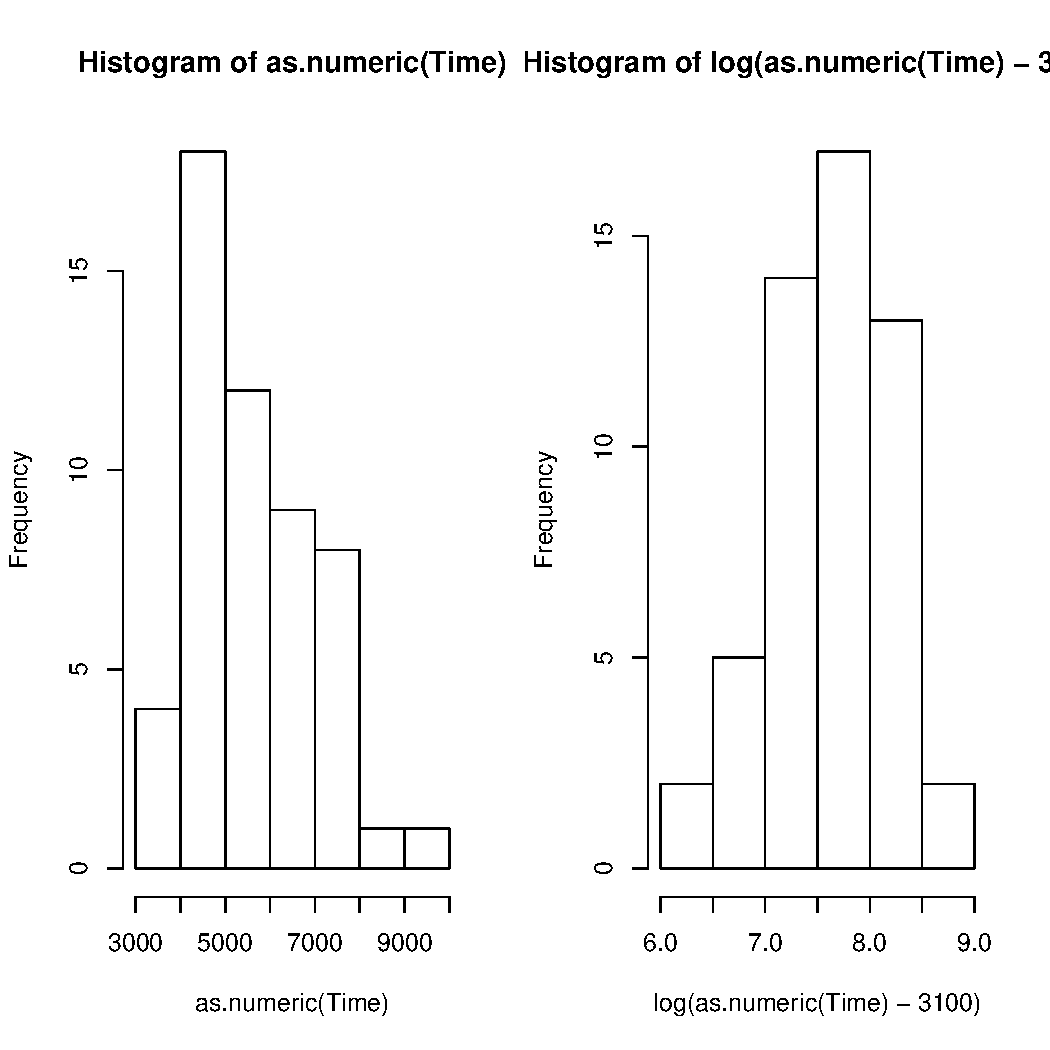
\includegraphics[width=9cm]{prob2a.pdf}
\caption{\label{fig:prob2a}Histograms of Time and Log(Time - 3100)}
\end{figure}
\subsection{Plot a scatterplot log(Time - 3100) vs. Year}
\label{sec-3-3}



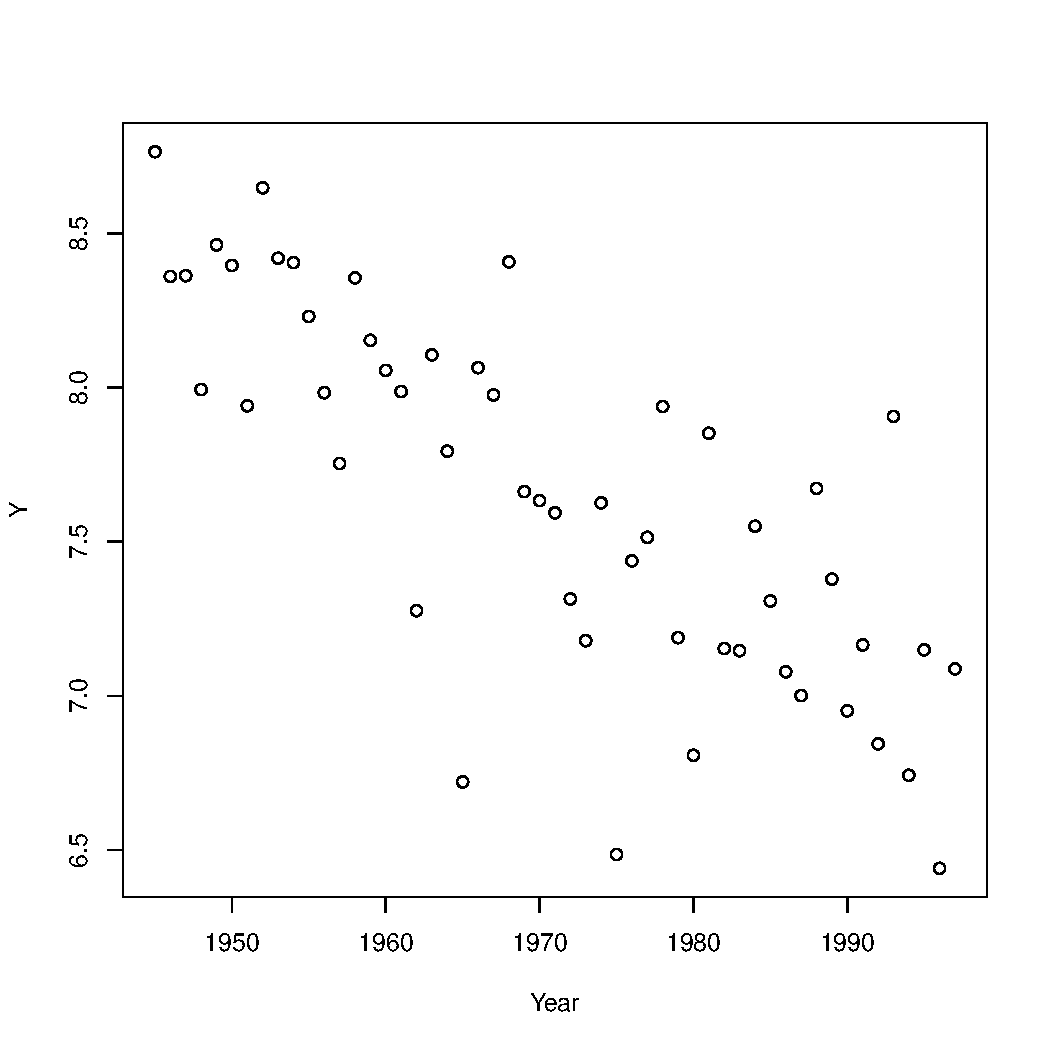
\includegraphics[width=.9\linewidth]{prob2b.pdf}
\subsubsection{Write out a linear model to study the relationship between log(Time - 3100) and Year.}
\label{sec-3-3-1}

Interpret your two parameters in the model.

\begin{align*}
\mathrm{Let} Y_i &= log(\mathrm{Time}_i -3100)\\
\mathrm{Model:} Y_i = \beta_0 + \beta_1 X_i + \epsilon_i\\
\hat{\beta}_1 &= \frac{S_{xy}}{S_{xx}} \\
              &=\frac{ \sum (X_i - \bar{X})(Y_i - \bar{Y})}{\sum (X_i - \bar{X})^2}\\
              &= -0.03\\
\hat{\beta}_{0} &= \bar(Y) - \hat{\beta}_{1}\bar{X}\\
              &= 65.64
\end{align*}

\textbf{Interpretation:} $\beta$$_0$ tells us the value of Y when/if X equals 0.
So in year 0, we would expect $\log(\mathrm{Time} - 3100)$ to be
approximately 66. Solving for Time gives \texttt{3.2226970275426e+28}.

$\beta$$_1$ tells us the magnitude of increase in $\log(\mathrm{Time} -
3100)$ for a 1 year increase in time. Since $\beta$$_0$ is negative, it
is actually a decrease. Solving for Time gives \texttt{3100.97}
\section{Problem 3 Matrix Practice}
\label{sec-4}




 % latex table generated in R 3.0.2 by xtable 1.7-4 package
% Fri Jan  9 13:53:21 2015
\begin{bmatrix}{}
  1.00 & -4.00 \\ 
  -3.00 & 0.00 \\ 
  2.00 & -3.00 \\ 
  \end{bmatrix}

\end{document}
